\documentclass[border=8pt]{standalone}
\usepackage{fontspec}
\setmainfont[
  Path = ../fonts/,
  UprightFont = Cabin-Regular.ttf,
  BoldFont = Cabin-Bold.ttf,
  ItalicFont = Cabin-Italic.ttf
]{Cabin}
\usepackage{amsmath, amssymb}
\usepackage{tikz}
\usetikzlibrary{arrows.meta, positioning, shapes.geometric, calc}

\begin{document}
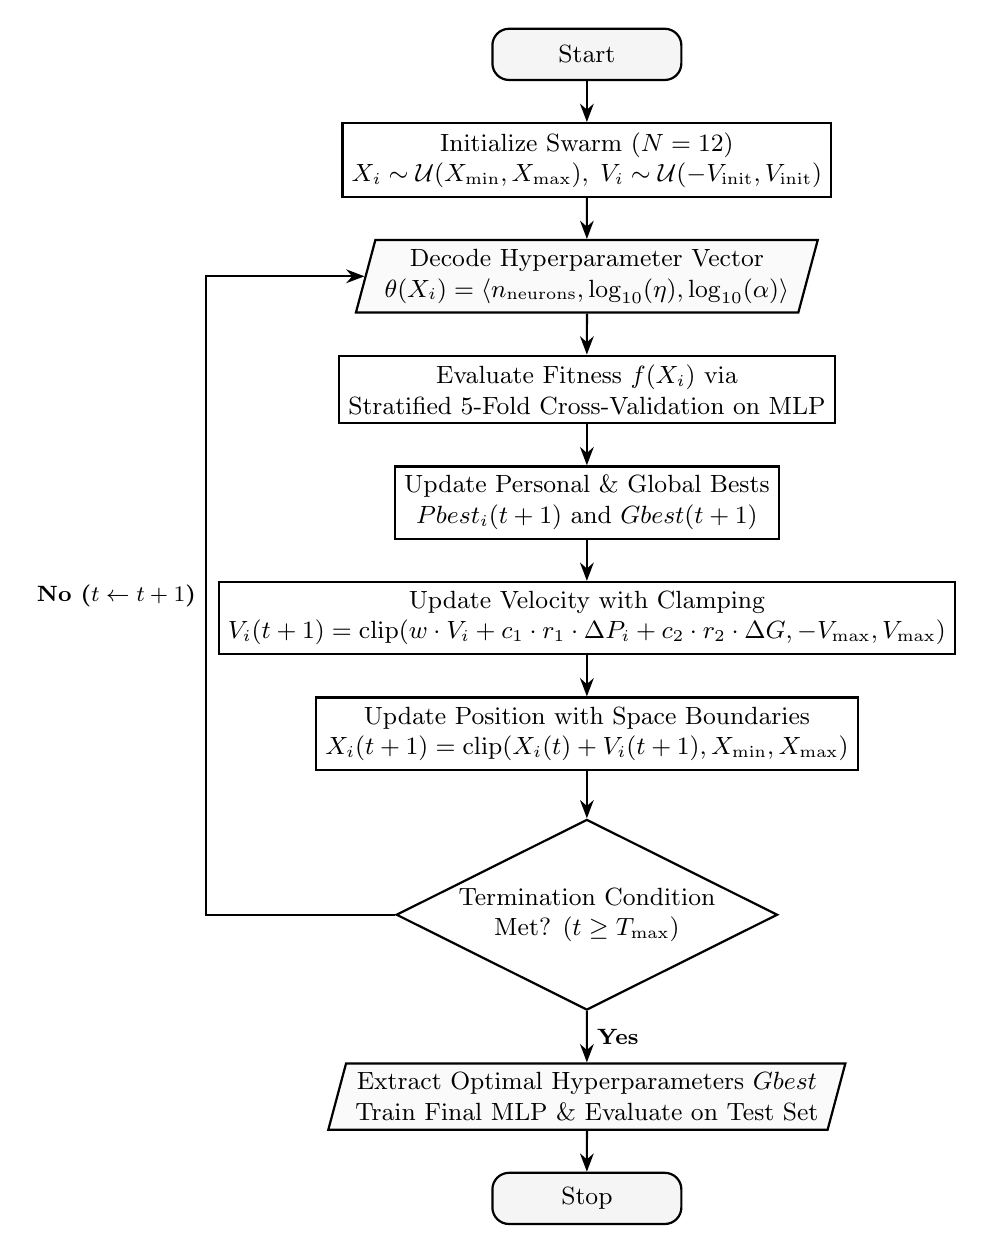
\begin{tikzpicture}[
    font=\fontsize{9pt}{11pt}\selectfont,
    >=Stealth,
    node distance=0.52cm,
    startstop/.style={draw, rounded corners=6pt, fill=black!4, minimum width=2.4cm, minimum height=0.65cm, align=center, line width=0.8pt},
    process/.style={draw, rectangle, fill=white, minimum width=4.0cm, minimum height=0.72cm, align=center, line width=0.8pt},
    data/.style={draw, trapezium, trapezium left angle=75, trapezium right angle=105, fill=black!2, minimum width=3.4cm, minimum height=0.68cm, align=center, line width=0.8pt},
    decision/.style={draw, diamond, aspect=2.0, fill=white, minimum width=2.6cm, minimum height=0.8cm, align=center, line width=0.8pt, inner sep=1pt}
]

% Main Flow Column
\node (start) [startstop] {Start};
\node (init) [process, below=of start] {Initialize Swarm ($N=12$)\\$X_i \sim \mathcal{U}(X_{\min}, X_{\max}), \; V_i \sim \mathcal{U}(-V_{\mathrm{init}}, V_{\mathrm{init}})$};
\node (decode) [data, below=of init] {Decode Hyperparameter Vector\\$\theta(X_i) = \langle n_{\mathrm{neurons}}, \log_{10}(\eta), \log_{10}(\alpha) \rangle$};
\node (cv_eval) [process, below=of decode] {Evaluate Fitness $f(X_i)$ via\\Stratified 5-Fold Cross-Validation on MLP};
\node (update_best) [process, below=of cv_eval] {Update Personal \& Global Bests\\$Pbest_i(t+1)$ and $Gbest(t+1)$};
\node (update_vel) [process, below=of update_best] {Update Velocity with Clamping\\$V_i(t+1) = \mathrm{clip}(w \cdot V_i + c_1 \cdot r_1 \cdot \Delta P_i + c_2 \cdot r_2 \cdot \Delta G, -V_{\max}, V_{\max})$};
\node (update_pos) [process, below=of update_vel] {Update Position with Space Boundaries\\$X_i(t+1) = \mathrm{clip}(X_i(t) + V_i(t+1), X_{\min}, X_{\max})$};
\node (term) [decision, below=0.6cm of update_pos] {Termination Condition\\Met? ($t \ge T_{\max}$)};
\node (output) [data, below=0.65cm of term] {Extract Optimal Hyperparameters $Gbest$\\Train Final MLP \& Evaluate on Test Set};
\node (stop) [startstop, below=of output] {Stop};

% Arrows
\draw[->, line width=0.8pt] (start) -- (init);
\draw[->, line width=0.8pt] (init) -- (decode);
\draw[->, line width=0.8pt] (decode) -- (cv_eval);
\draw[->, line width=0.8pt] (cv_eval) -- (update_best);
\draw[->, line width=0.8pt] (update_best) -- (update_vel);
\draw[->, line width=0.8pt] (update_vel) -- (update_pos);
\draw[->, line width=0.8pt] (update_pos) -- (term);
\draw[->, line width=0.8pt] (term) -- node[right, font=\footnotesize\bfseries] {Yes} (output);
\draw[->, line width=0.8pt] (output) -- (stop);

% Feedback Loop with ample clearance
\draw[->, line width=0.8pt] (term.west) -- ++(-2.4,0) |- node[pos=0.25, left, font=\footnotesize\bfseries] {No ($t \leftarrow t+1$)} (decode.west);

\end{tikzpicture}
\end{document}
